\newpage
IRSTI 61.31.40

\sectionwithauthors{M.K. Kazankapova, B.T. Yermagambet, G.K. Mendaliyev, A. Samatkyzy, A.B. Malgazhdarova}{OBTAINING CARBON NANOMATERIALS FROM SHUBARKOL COAL AND
APPLICATION FOR HYDROGEN STORAGE}

\begin{center}
{\bfseries \textsuperscript{1,2,3}M.K. Kazankapova, \textsuperscript{1,2}B.T. Yermagambet, \textsuperscript{1,2}G.K. Mendaliyev, \textsuperscript{1}A. Samatkyzy, \textsuperscript{1,2}A.B. Malgazhdarova}

\textsuperscript{1}«Institute of Coal Chemistry and Technology» LLP,
Astana, Kazakhstan,

\textsuperscript{2}L.N. Gumilyov Eurasian National University{\bfseries ,}
Astana, Kazakhstan,

\textsuperscript{3}Kazakh university of technology and business named
after K. Kulazhanov, Astana, Kazakhstan

Corresponding author: е-mail: coaltech@bk.ru
\end{center}

This study presents a promising method for the synthesis of graphene -
the electric arc discharge method. The synthesis of nanomaterials
containing graphene was carried out based on carbonized coal "Shubarkol"
using the electric arc discharge method at a constant voltage of 75 V
and a current of 100 A in a quartz reactor. Based on Raman scattering
data and analysis of electrical properties (dielectric constant and
electrical resistance), it was shown that the synthesized products have
a high degree of graphitization and long-range structural order (2D
peak), which indicates the formation of nanomaterials containing
graphene. These results present a potential route for low-cost mass
production of high-quality graphene samples. In addition, the electrical
resistance (R), capacitance (C) and dielectric constant (ε), electrical
resistivity (R) and electrical conductivity (χ) of nanomaterials
containing graphene were determined for the first time in the
temperature range 293-483 K. The highest a degree of graphitization of
80.7\% is achieved with the formation of graphene-containing material on
the walls of the reactor after an arc discharge. Since the resulting
nanomaterial on the reactor walls showed better results in terms of
physicochemical and electrophysical properties, the material was tested
for hydrogen storage. The sorption capacity of the nanomaterial for
hydrogen was 35.1516 cm\textsuperscript{3}/g (0.314\%).

{\bfseries Key words:} coal, carbonized coal, carbon nanotubes, graphene,
arc discharge, hydrogen, storage.

\sectionheading{ШҰБАРКӨЛ КӨМІРІНЕН КӨМІРТЕК НАНОМАТЕРИАЛДАРЫН АЛУ ЖӘНЕ СУТЕКТІ
САҚТАУҒА ҚОЛДАНУ}

\begin{center}
{\bfseries \textsuperscript{1,2,3}М.Қ. Қазанқапова,
\textsuperscript{1,2}Б.Т. Ермағамбет, \textsuperscript{1,2}Ғ.К.
Мендалиев, \textsuperscript{1}Ә. Саматқызы,}

{\bfseries \textsuperscript{1,2}А.Б.Малғаждарова}

\textsuperscript{1}«Көмір химиясы және технология институты» ЖШС,
Астана, Қазақстан,

\textsuperscript{2}Л.Н. Гумилев атындағы Еуразия ұлттық университеті,
Астана, Қазақстан,

\textsuperscript{3}Қ.Құлажанов атындағы Қазақ технология және бизнес
университеті, Астана, Қазақстан,

е-mail: coaltech@bk.ru
\end{center}

Бұл зерттеуде графен синтезінің перспективті әдісі - электр доғалық
разряд әдісі ұсынылды. Құрамында графен бар наноматериалдардың синтезі
кварц реакторында 75 В тұрақты кернеуде және 100 А ток кезінде электр
доғалық разряд әдісін қолдану арқылы «Шұбаркөл» көмірі негізінде жүзеге
асырылды. Раман шашырау деректері және электрлік қасиеттерді талдау
(диэлектрлік өтімділік және электр кедергісі) негізінде синтезделген
өнімдерде графиттенудің жоғары дәрежесі және алысдиапазондағы құрылымдық
реті (2D шыңы) бар, бұл құрамында графен бар наноматериалдардың түзілуін
көрсетеді. Бұл нәтижелер жоғары сапалы графен үлгілерін арзан жаппай
өндірудің әлеуетті бағытын көрсетеді. Сонымен қатар, құрамында графен
бар наноматериалдардың электрлік кедергісі (R), сыйымдылығы (C) және
диэлектрлік өтімділігі (ε), электрлік кедергісі (R) және электр
өткізгіштігі (χ) 293-483 К температура диапазонында алғаш рет анықталды.
Графиттенудің ең жоғары дәрежесі 80,7\% доғалық разрядтан кейін
реактордың қабырғаларында графен бар материалдың пайда болуымен қол
жеткізіледі. Реактор қабырғаларында алынған наноматериал физика-химиялық
және электрофизикалық қасиеттері бойынша жақсы нәтиже көрсеткендіктен,
материал сутегі сақтау үшін сынақтан өтті. Наноматериалдың сутегі үшін
сорбциялық қабілеті 35,1516 см\textsuperscript{3}/г (0,314\%) құрады.

{\bfseries Түйін сөздер:} көмір, көміртекті көмір, көміртекті нанотүтіктер,
графен, доғалық разряд, сутегі, сақтау.

\sectionheading{ПОЛУЧЕНИЕ УГЛЕРОДНЫХ НАНОМАТЕРИАЛОВ ИЗ ШУБАРКОЛЬСКОГО УГЛЯ И
ПРИМЕНЕНИЕ ДЛЯ ХРАНЕНИЯ ВОДОРОДА}

\begin{center}
{\bfseries \textsuperscript{1,2,3}М.К. Казанкапова,
\textsuperscript{1,2}Б.Т. Ермағамбет, \textsuperscript{1,2}Г.К.
Мендалиев, \textsuperscript{1}А. Саматкызы, \textsuperscript{1,2}Б А.Б.
Малгаждарова}

\textsuperscript{1}ТОО «Институт химии угля и технологии», Астана,
Казахстан,

\textsuperscript{2}Евразийский национальный университет им. Л.Н.
Гумилева, Астана, Казахстан,

\textsuperscript{3}Казахский университет технологии и бизнеса имени
К.Кулажанова, Астана, Казахстан,

е-mail: coaltech@bk.ru
\end{center}

В данном исследовании представлен перспективный метод синтеза графена -
метод электродугового разряда. Был осуществлен синтез наноматериалов,
содержащих графен, на основе карбонизованного угля «Шубарколь» с
использованием метода электродугового разряда при постоянном напряжении
75 В и токе 100 А в кварцевом реакторе. На основе данных метода
комбинационного рассеяния света и анализа электрофизических свойств
(диэлектрической проницаемости и электрического сопротивления) было
показано, что синтезированные продукты обладают высокой степенью
графитизации и дальним порядком структуры (2D пик), что свидетельствует
о формировании наноматериалов, содержащих графен. Эти результаты
представляют потенциальный путь для дешевого массового производства
высококачественных образцов графена. Кроме того, впервые были определены
электрическое сопротивление (R), емкость (C) и диэлектрическая
проницаемость (ε), удельное электрическое сопротивление (R) и удельная
электропроводность (χ) наноматериалов, содержащих графен, в интервале
температур 293-483 К. Самая высокая степень графитизации 80,7\%
достигается при образовании графенсодержащего материала на стенках
реактора после дугового разряда. Поскольку полученный наноматериал на
стенках реактора показал лучшие результаты по физико-химическим и
электрофизическим свойствам, материал был протестирован на хранение
водорода. Сорбционная емкость наноматриала по водороду составила -
35.1516 см\textsuperscript{3}/г (0.314\%).

{\bfseries Ключевые слова:} уголь, карбонизованный уголь, углеродные
нанотрубки, графен, дуговой разряд, водород, хранение.

\begin{multicols}{2}
{\bfseries Introduction.} Since Sumio Iijima reported it in 1991, carbon
nanotubes (CNTs) have attracted much attention from researchers and
industry. CNTs can be classified into single-walled CNTs (SWNTs),
double-walled CNTs (DWNTs), and multi-walled CNTs (MWNTs) depending on
the number of graphite layers. They consist of sp\textsuperscript{2}
bonded carbon atoms arranged in a cylindrical tube ranging in length
from less than 100 nm to several centimeters. The diameter of SWCNTs is
typically 0.4--2 nm, while the diameter of MWCNTs ranges from *1.4 nm to
nearly 100 nm, depending on the synthesis conditions. CNTs are well
known for their unique physicochemical properties, including extremely
high tensile strength, high electrical conductivity, high ductility, and
relative chemical inactivity. All these properties make CNT-based
products attractive. Moreover, due to their low dimensionality, CNTs are
also preferred for use in the development of nanocomposites. In this
context, CNTs open up a new direction in materials science and
nanotechnology. CNTs can be found in a wide range of applications, such
as electronics, polymer composites, energy storage materials, catalysis,
gas storage materials and sensors {[}1{]}.

There are many methods for synthesizing nanostructures. They are usually
divided into two groups: «Top bottom» is a «top-down» technology, that
is, the dispersion of macroscopic bodies into nanoscale sizes, and the
second group «bottom-up» is a technology the assembly of nanoparticles
from atoms. There are also various hybrid methods.

One of the first methods for producing carbon nanoparticles was laser
evaporation of graphite or coal, arc evaporation of graphite in the
presence of a metal catalyst, chemical vapor deposition, pyrolysis, and
mechanical separation {[}2{]}.

Arc discharge is the oldest and most common method for producing CNM.
This also makes it possible to obtain carbon formed by fullerene and
soot molecules. This method is based on the electrical destruction of
gas to produce plasma. It uses high temperature (over 1700°C) to
evaporate carbon atoms in plasma, allowing CNMs to grow with fewer
structural defects than other methods.

The chamber consists of two electrodes, one of which is the anode and
the other is the cathode. The anode is filled with a mixture of graphite
powder and catalyst. The catalyst promotes the growth of SWCNTs rather
than MWCNTs {[}3{]}. The cathode consists of a pure graphite rod.
Initially, the electrodes are held independently of each other in a gas
atmosphere (usually an argon/hydrogen mixture); then the distance
between the electrodes is reduced, and an electric arc is applied with
an intensity of 60-100 A or 50-150 A, which corresponds to a decrease in
potential by 25 V {[}4, 5{]}.

The inert gas flow is maintained at 50-600 Torr; the temperature in the
interelectrode region ranges from 1700° to 4000 °C. The electrodes turn
red and plasma is formed, so carbon sublimes from the positive anode,
which is consumed and condenses as a filamentary carbon product at the
cathode due to the temperature gradient.

Speaking about the physical and chemical properties of carbon nanotubes,
CNTs are the strongest and hardest materials on earth in terms of
tensile strength and elastic modulus. The planar cellular carbon atoms
of graphene in CNTs are responsible for these high-strength fibers.
Carbon nanotube is more rigid than steel and is very resistant to
physical damage.

When you press on the end of the nanotube, it bends without damaging the
tip, and when the force is removed, the tip returns to its original
position. The reason they don\textquotesingle t break is because the
carbon rings of the walls change their structure when bent, but
don\textquotesingle t break. This is a unique result of sp2 C-C bond
hybridization and bending overhybridization. The degree of change and
s-p coefficients depend on how much the bonds bend. Due to this
property, CNTs can be used as very high resolution probe tips for
scanning probe microscopy {[}6{]}.

In the metallic state, the conductivity of nanotubes is very high. They
can transmit billions of amps per square centimeter. Copper wire fails
when it transmits a million amps per square centimeter because the
joules of heat cause the wire to melt. Theoretically, metal nanotubes
can conduct an electric current density of 10-15
A/cm\textsuperscript{2}, which is 1000 times greater than that of metals
such as copper {[}7{]}. One of the reasons for the high conductivity of
carbon nanotubes is the very small number of defects that cause electron
scattering and therefore low resistance {[}8{]}.

Another carbon nanomaterial that can be synthesized by an arc discharge
is graphene {[}9-10{]}. Graphene is a material that has a large specific
surface area (2630 m2g-1), high internal mobility (200,000
cm\textsuperscript{2} V\textsuperscript{-1}s\textsuperscript{-1}), high
Young\textquotesingle s modulus (\textasciitilde{} 1.0 TPa), thermal
conductivity (\textasciitilde5000
W*m\textsuperscript{-1}/K\textsuperscript{-1}), optical transmittance
(\textasciitilde{} 97.7\%) {[}11-12{]}. In addition to arc, there are
methods of micromechanical cleavage, electrochemical exfoliation,
solvent-based exfoliation {[}13{]}, graphite oxide exfoliation {[}14{]}
and laser evaporation. Among all these methods, arc discharge has many
advantages such as low production cost, high efficiency, and the ability
to be synthesized without using any catalysis {[}15{]}.

In the research, multiple layers of graphene were synthesized using a
homemade arc discharge chamber. Helium (He), nitrogen (N), and mixtures
thereof have been used to understand the influence of the reactor
atmosphere on graphene synthesis. The purity and number of graphene
layers were determined using Raman spectroscopy. The purity of the
synthesized graphene also depends on the diameter of the electrodes and
the arc current. Thus, optimal synthesis conditions were obtained with
an electrode diameter of 12 mm and an arc current of 150 A in a
He+N\textsubscript{2} atmosphere. TEM studies revealed a crumpled
texture of graphene {[}16{]}.

Graphene can be doped with atoms of other elements, such as nitrogen,
fluorine, hydrogen, oxygen, etc., changing its properties. All this
makes it an interesting material for many applications. First of all,
these are applications in opto- and nanoelectronics (touch screens,
solar cells, flexible electronic devices, high-frequency transistors,
logic transistors), photonics (photodetectors, optical modulators,
mode-locked lasers, THz generators and optical polarizers), composite
materials, paints and coatings. Graphene is seen as a promising
candidate to replace transparent indium tin oxide (ITO) electrodes.
Promising applications of graphene coating include transparent heating
elements and thermoacoustic transducers.

{\bfseries Materials and methods.} In this work, carbon nanomaterials
obtained by the electric arc method were studied. Activated carbon
«Shubarkol» is used as an electrode. The coal carbonization process
includes an initial low-temperature (at 180°C, with a heating rate of
10°C/min) treatment of the raw material in the presence of air for 1
hour, followed by carbonization in an inert atmosphere at temperatures
ranging from 180-900°C with a heating rate of 5°C/min, and steam
activation at the maximum temperature for 1 hour. Process parameters:
constant voltage - 75 V; current -- \hspace{0pt}\hspace{0pt}100 A;
process time \textasciitilde10 min, inert gas - N\textsubscript{2} with
a purity of 99.99\%. The reactor is transparent quartz glass that can
withstand high temperatures. The chamber is placed inside the water used
for cooling. The principle of this method is the evaporation of carbon
under reduced pressure of an inert gas. According to the method scheme,
a movable anode and a stationary cathode are used, as in Fig. 1.
\end{multicols}

\begin{figure}[H]
	\centering
	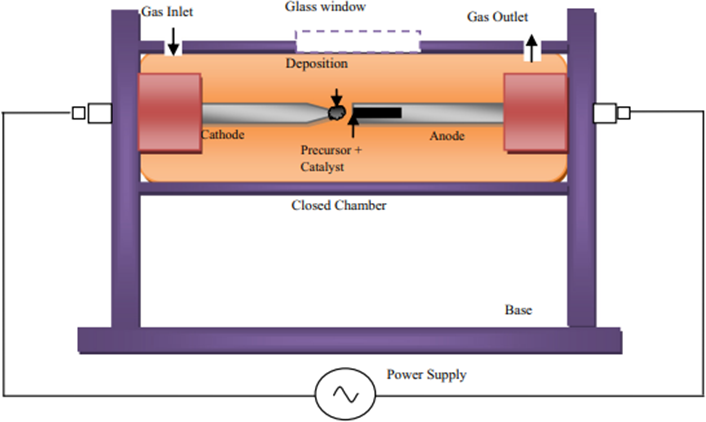
\includegraphics[width=0.8\textwidth]{assets/53}
	\caption*{Figure 1 - Schematic diagram of an electric arc discharge}
\end{figure}

\begin{multicols}{2}
After the electric arc is ignited, the plasma ignites. Carbon
nanomaterials condensed on the walls of the reactor and on the surface
of the electrode. Activated carbon "Shubarkol" after an arc discharge
was separated according to figure 2.

The resulting materials were tested for hydrogen storage at a
high-performance automatic physiosorption and chemisorption station
Micromeritics 3Flex Chemi\&TCD (Made in the USA). This device is
equipped with three ports, each of which has a 0.1 Torr sensor for
analysis of micropores. Before measurement, all samples were
preliminarily degassed using a SmartVacPrep unit (manufactured by
Micromeritics, USA) equipped with a forevacuum pump.
\end{multicols}

\begin{figure}[H]
	\centering
	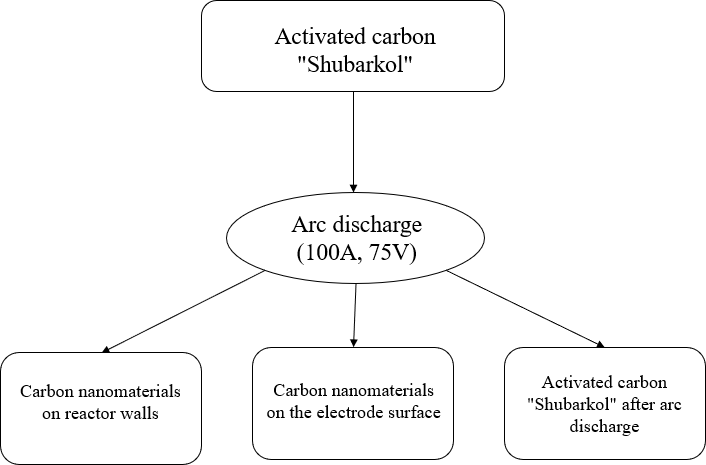
\includegraphics[width=0.8\textwidth]{assets/54}
	\caption*{Figure 2 - Schematic diagram for producing nanomaterials using the electric arc discharge method}
\end{figure}

\begin{multicols}{2}
Adsorbate gas - hydrogen, measurement temperature - 77 K,
p\textsubscript{0} values \hspace{0pt}\hspace{0pt}for all points were
considered the same and equal to 760 Torr, A Peak Scientific hydrogen
generator with a maximum productivity of 500 cm\textsuperscript{3}/min
was used as a source of hydrogen, Water in the hydrogen generator was
used from a Thermo Scientific deionizer, Readout points started from a
value of 0.0001 p/p\textsubscript{0} to 0.995 p/p\textsubscript{0}. The
measurement of free space or void volume was carried out after analysis
with helium in order to avoid premature filling of micropores with
helium.

Due to the smaller radius and transverse radius of the hydrogen
molecule, the specific surface area and porosity values
\hspace{0pt}\hspace{0pt}will be higher compared to nitrogen sorption.
Classical BET methods in the case of H\textsubscript{2} will be
incorrect since the saturation pressure value was used as a constant
(760 Torr). To calculate the pore distribution, the theoretical hydrogen
sorption model DFT HS H\textsubscript{2} Carbon, heterogeneous, taking
into account the heterogeneity of the carbon surface. For most samples,
this model showed good consistency. The limitation of nitrogen to fill
pores with a radius of less than 0.35 nm was also taken into account.

{\bfseries Results and discussion.} The obtained materials were studied by
SEM and Raman spectroscopy. As a result, the original «Shubarkol» coal
contained different agglomerates ranging from 719 nm to 231.97 µm, as
shown in Fig. 3. The degree of graphitization is G\textsubscript{f} =
29.6\% and peaks at 1258.3 are noticeable; 1374.9; 1535.1; 1594.3;
2704.9; 2928.6 cm\textsuperscript{-1}. I(D)/I(G)=0.6 I(G)/I(2D)=12.2.
The intensity of peak D at 1374.9 cm\textsuperscript{-1} is lower than
peak G at 1594.3 cm\textsuperscript{-1}, and peak G at 1594.3
cm\textsuperscript{-1} is much higher than peak 2D at 2704.9
cm\textsuperscript{-1} (Figure 4), this explains that the material is
amorphous carbon. There may be polymer chains or other impurities, as
indicated by the luminescent trend.
\end{multicols}

\begin{figure}[H]
	\centering
	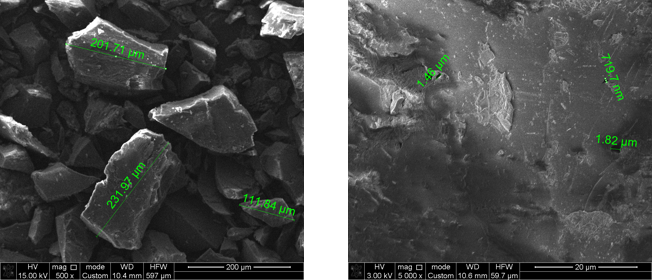
\includegraphics[width=0.8\textwidth]{assets/55}
	\caption*{Figure 3 - SEM of the original coal «Shubarkol»}
\end{figure}

\begin{figure}[H]
	\centering
	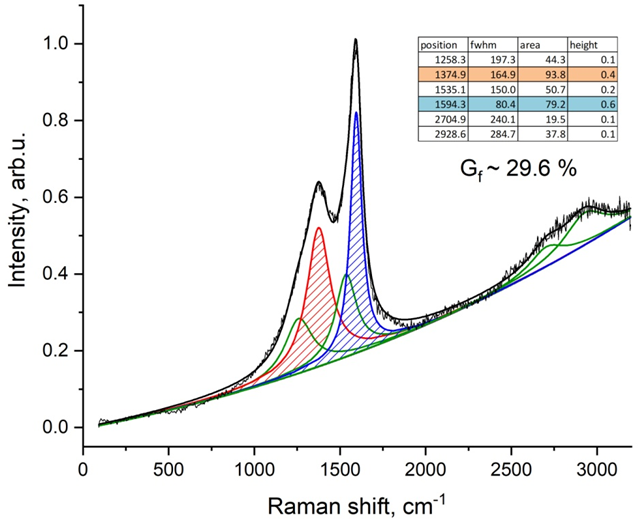
\includegraphics[width=0.7\textwidth]{assets/56}
	\caption*{Figure 4 - Raman spectroscopy of the original coal «Shubarkol»}
\end{figure}

\begin{multicols}{2}
After activation of Shubarkol coal, SEM images show that agglomerates of
different elements were removed. Pores are noticeable, with sizes
ranging from 155 nm to 33.08 µm. During the carbonization process,
mineral agglomerates opened, as shown in Fig. 5 by white spots. Peaks at
1194.4 are visible in the Raman spectrum; 1347.9; 1517.1; 1595.4;
2700.7; 2914.0 cm\textsuperscript{-1}. The degree of graphitization
after the activation process dropped to G\textsubscript{f}=24\%, this is
explained by the fact that peak D 1347.9 cm\textsuperscript{-1}
increased its intensity (Figure 6). I(D)/I(G)=0.9 I(G)/I(2D)=13.1.
Amorphous carbon with signs of graphitization - a narrow peak G, as well
as a weak manifestation of a second-order peak - 2D.
\end{multicols}

\begin{figure}[H]
	\centering
	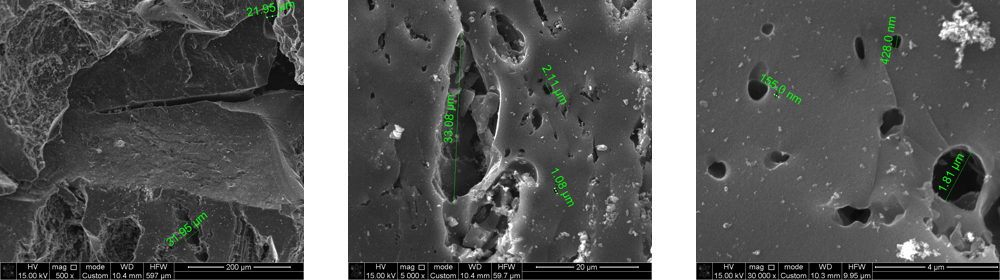
\includegraphics[width=0.9\textwidth]{assets/57}
	\caption*{Figure 5 - SEM image of activated carbon «Shubarkol»}
\end{figure}

\begin{figure}[H]
	\centering
	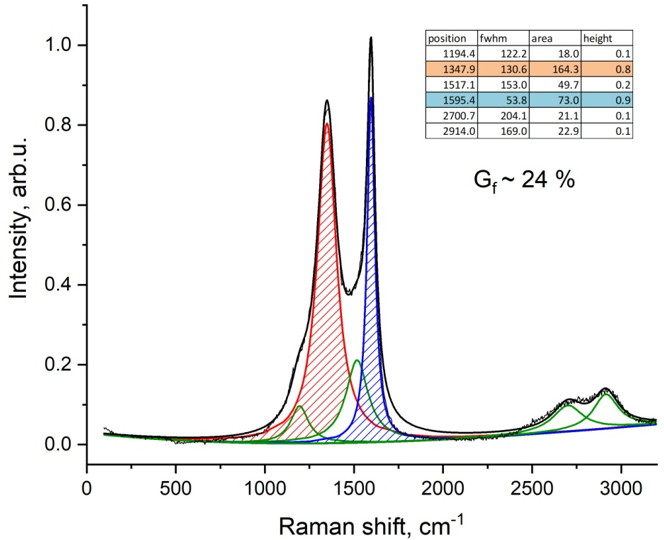
\includegraphics[width=0.7\textwidth]{assets/58}
	\caption*{Figure 6 - Raman spectroscopy of activated carbon «Shubarkol»}
\end{figure}

\begin{multicols}{2}
After the arc discharge, we see deformation of the pores in SEM images.
The pores have become smaller and range from 159.9 nm to 1.83 µm. The
formation of micro- and mesopores is assumed. White flake-like spots are
visible on the surface (Figure 7). As you can see in Fig. 8 there are
peaks at 1363.7(D); 1465; 1582.5(G); 2448.5; 2725.9(2D); 2959
cm\textsuperscript{-1} According to the Raman spectroscopy data, the
«Shubarkol» activated carbon after an arc discharge on the reactor walls
has a high degree of graphitization G\textsubscript{f} = 80.7\%.
Compared with activated carbon, peak D shows a weaker intensity, and
peak 2D shows a more prominent intensity. I(D)/I(G)=0.1, I(G)/I(2D)=2.9.
As a result, it can be said from the surface of the «Shubarkol»
activated carbon that after an arc discharge, graphene structures of
high quality and small thickness were formed on the walls of the
reactor.
\end{multicols}

\begin{figure}[H]
	\centering
	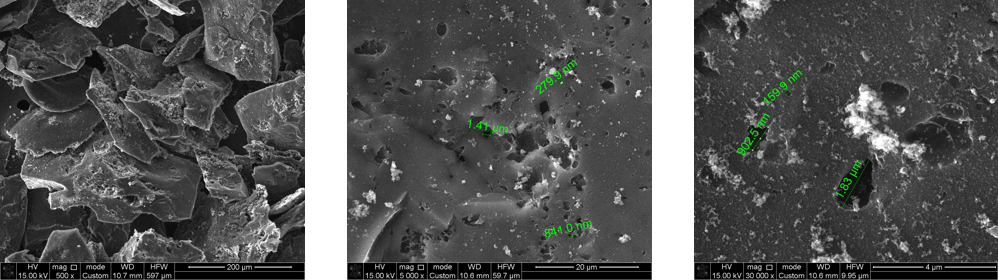
\includegraphics[width=0.9\textwidth]{assets/59}
	\caption*{Figure 7 - SEM image of «Shubarkol» activated carbon after an arc discharge on the walls of the reactor (100A, 75B)}
\end{figure}

\begin{figure}[H]
	\centering
	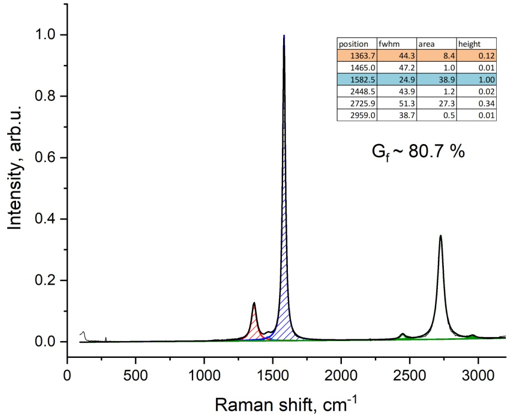
\includegraphics[width=0.7\textwidth]{assets/60}
	\caption*{Figure 8 - Raman spectroscopy of «Shubarkol» activated carbon after an arc discharge on the walls of the reactor (100A, 75B)}
\end{figure}

\begin{multicols}{2}
After an arc discharge, layers of graphene are visible on the surface of
the Shubarkol coal, according to the SEM image. Nanomaterials ranging in
size from 67.3 nm to 467.9 nm were formed. Pore
\hspace{0pt}\hspace{0pt}deformations are noticeable (Fig. 9). It is
assumed that layers of graphene have grown together on the surface of
the pores. In the Raman peaks at 1228.8 are noticeable; 1355.3(D);
1476.6; 1577.4(G); 2435.4; 2714.5(2D); 2935 cm\textsuperscript{-1}.
I(D)/I(G)=0.3 I(G)/I(2D)=2.8 From these data we can say that on the
surface of the Shubarkol activated carbon after an arc discharge on the
surface of the electrode there are graphene-like structures of varying
degrees of defects (Fig. 10).
\end{multicols}

\begin{figure}[H]
	\centering
	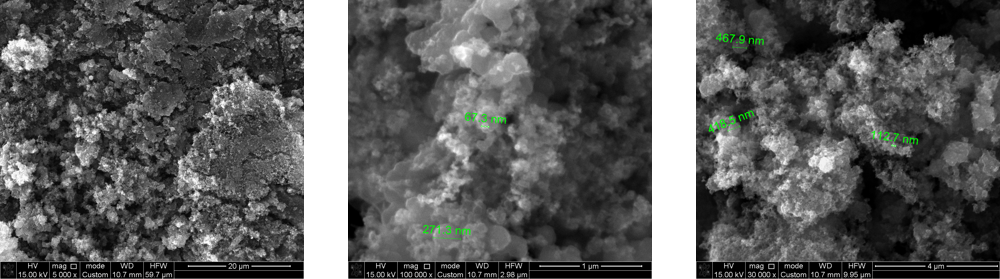
\includegraphics[width=0.9\textwidth]{assets/61}
	\caption*{Figure 9 - SEM image of activated carbon «Shubarkol» after an arc discharge on the surface of the electrode (100A, 75B)}
\end{figure}

\begin{figure}[H]
	\centering
	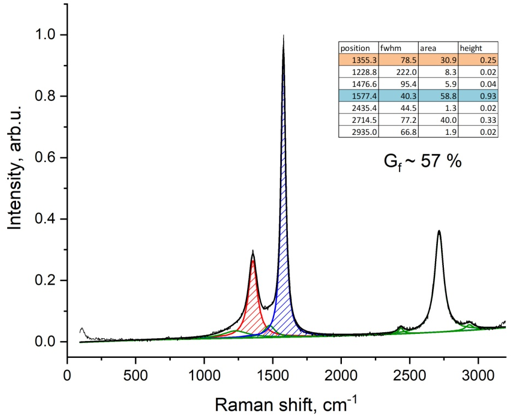
\includegraphics[width=0.7\textwidth]{assets/62}
	\caption*{Figure 10 - Raman spectroscopy of activated carbon «Shubarkol» after an arc discharge on the surface of the electrode (100A, 75B)}
\end{figure}

\begin{multicols}{2}
SEM images (Figure 11) of crushed Shubarkol coal used as an electrode
show nanodots of different diameters. The dots start from 29.5 nm to
8.95 µm. Peaks at 1249.1 are visible in the Raman distribution;
1357.4(D); 1472.6; 1584.6(G); 2459.1; 2725.3(D); 2937.4
cm\textsuperscript{-1}. I(D)/I(G)=0.4 I(G)/I(2D)=1.8. Graphene-like
structures of varying degrees of defects and thickness.
\end{multicols}

\begin{figure}[H]
	\centering
	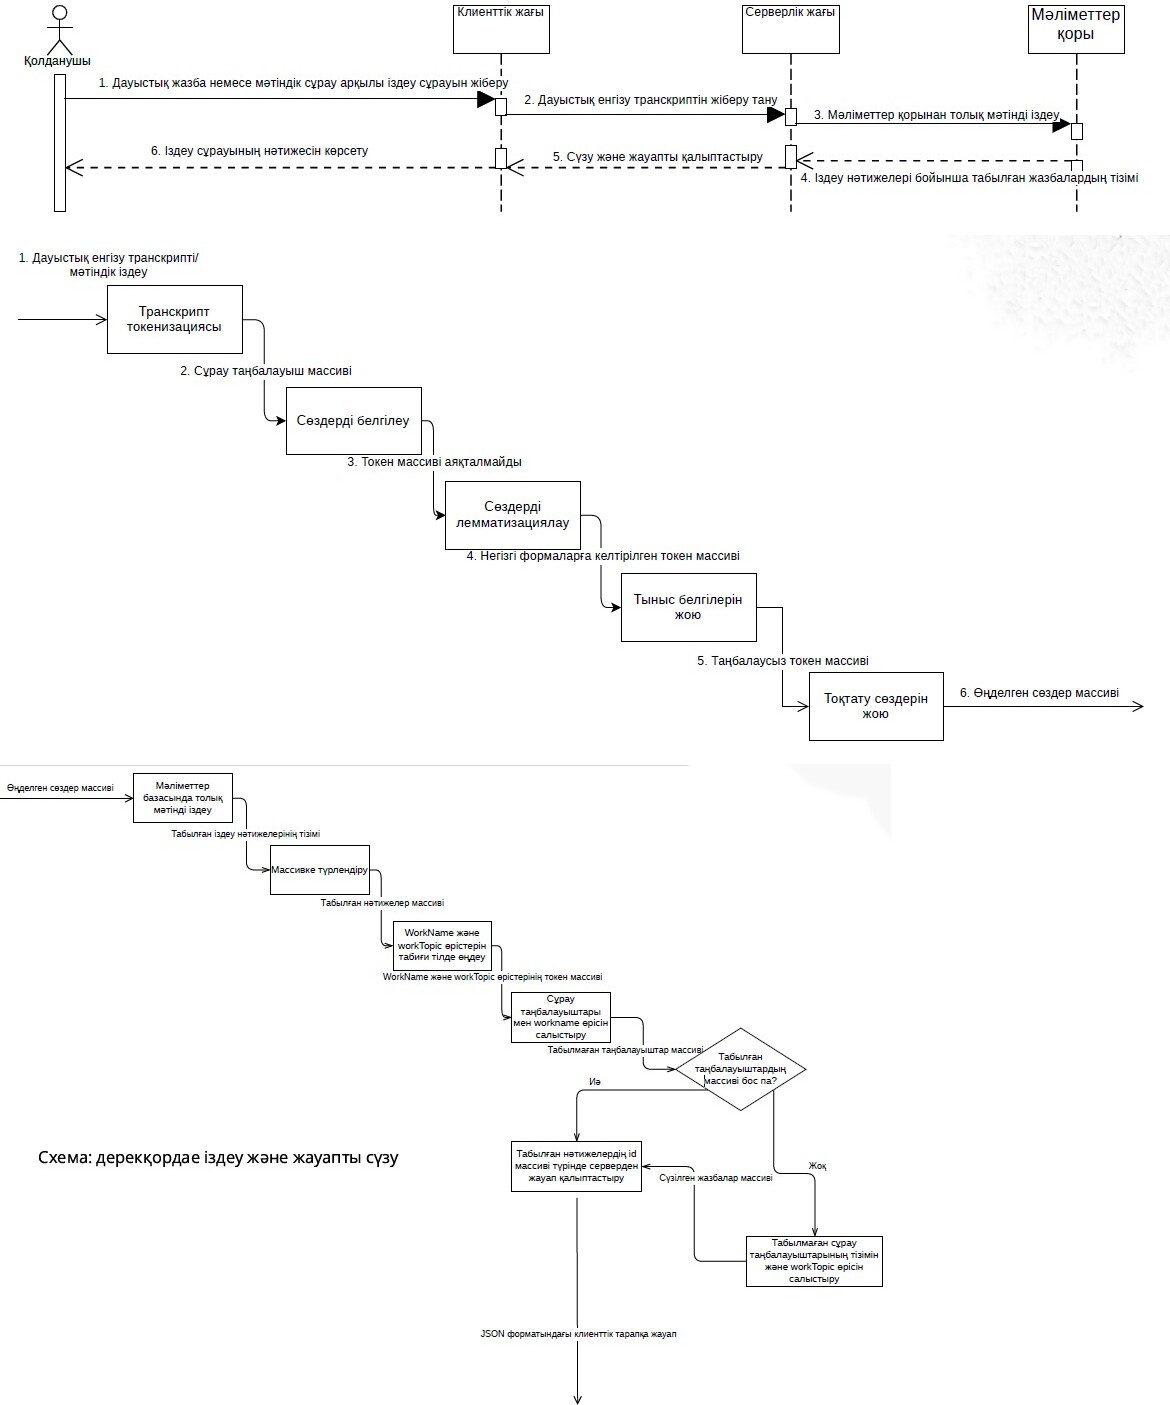
\includegraphics[width=\textwidth]{assets/63}
	\caption*{Figure 11 - SEM image of «Shubarkol» activated carbon after an arc discharge (100A, 75B)}
\end{figure}

\begin{figure}[H]
	\centering
	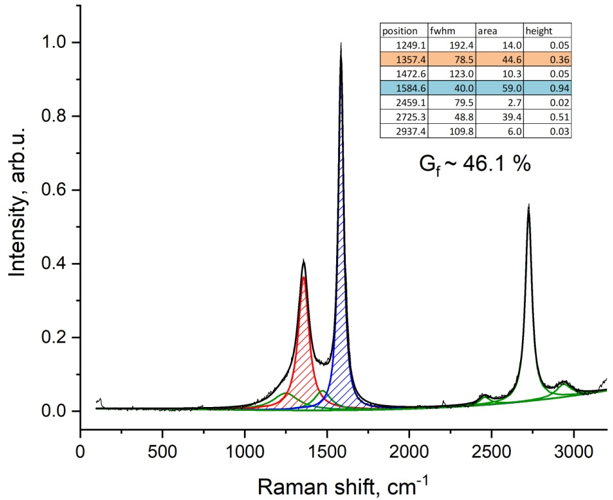
\includegraphics[width=0.7\textwidth]{assets/64}
	\caption*{Figure 12 - Raman spectroscopy of «Shubarkol» activated carbon after an arc discharge (100A, 75B)}
\end{figure}

\begin{multicols}{2}
It is known that the 2D band of Raman spectra is more sensitive to the
overlay of graphene sheets. From the Raman scattering data (Raman
effect), the intensities of the D, G and 2D peaks were calculated. It is
immediately noticeable that after activation the G peak increased its
intensity from 0.6 to 0.9. After the arc discharge, peak D loses its
intensity, and peak 2D increased its intensity from 0.1 to 0.51. The
intensity ratios I2D/IG for one-, two-, three- and multilayer
(\textgreater{} 4) in these materials were shown to vary from 0.11 to
0.54. And the ratio of IG/I2D peaks after arc treatment is from 1.84 to
2.94, which confirms the formation of two to three layer graphene (for
single-layer graphene the ratio is 0.6-1). The Raman spectrum of the
material with the lowest degree of crystallization contains a strong
D-band and a broad and weak G-band, and their high
\end{multicols}

\begin{table}[H]
\caption*{Table 1 - Ratio of D G and 2D peaks in materials obtained from Shubarkol coal}
\caption*{intensity ratio (ID/IG) confirms the strong disorder of the structure.
Based on the intensity ratio of the ID/IG bands after an arc discharge,
which ranges from 0.12 to 0.38, it can be argued that there are a small
number of material defects. Based on these data, we can say that we have
obtained modern carbon materials of very good quality.}
\centering
\begin{tabular}{|c|cc|cc|cc|cc|cc|}
\hline
\multirow{2}{*}{Elements} & \multicolumn{2}{p{0.1\textwidth}|}{Source coal «Shubarkol»} & \multicolumn{2}{p{0.13\textwidth}|}{Activated carbon «Shubarkol»} & \multicolumn{2}{p{0.15\textwidth}|}{Activated carbon «Shubarkol» After arcing (on the walls of the reactor)} & \multicolumn{2}{p{0.15\textwidth}|}{Activated carbon «Shubarkol» after arc discharge (on the surface of the electrode)} & \multicolumn{2}{p{0.15\textwidth}|}{Activated carbon  «Shubarkol» after an arc discharge (crushed electrode)} \\ \cline{2-11} 
 & \multicolumn{1}{c|}{Wt\%} & At\% & \multicolumn{1}{c|}{Wt\%} & At\% & \multicolumn{1}{c|}{Wt\%} & At\% & \multicolumn{1}{c|}{Wt\%} & At\% & \multicolumn{1}{c|}{Wt\%} & At\% \\ \hline
C & \multicolumn{1}{c|}{77,15} & 82 & \multicolumn{1}{c|}{90,35} & 92,92 & \multicolumn{1}{c|}{87,21} & 90,40 & \multicolumn{1}{c|}{71,70} & 85,89 & \multicolumn{1}{c|}{83,49} & 90,83 \\ \hline
O & \multicolumn{1}{c|}{22,24} & 17,74 & \multicolumn{1}{c|}{8,57} & 6,62 & \multicolumn{1}{c|}{11,75} & 9,15 & \multicolumn{1}{c|}{6,51} & 5,86 & \multicolumn{1}{c|}{7,84} & 6,40 \\ \hline
Al & \multicolumn{1}{c|}{0,4} & 0,19 & \multicolumn{1}{c|}{0,35} & 0,16 & \multicolumn{1}{c|}{0,36} & 0,16 & \multicolumn{1}{c|}{2,04} & 1,09 & \multicolumn{1}{c|}{0,6} & 0,29 \\ \hline
Si & \multicolumn{1}{c|}{0,07} & 0,03 & \multicolumn{1}{c|}{0,11} & 0,05 & \multicolumn{1}{c|}{0,19} & 0,08 & \multicolumn{1}{c|}{7,68} & 3,94 & \multicolumn{1}{c|}{0,44} & 0,21 \\ \hline
Ca & \multicolumn{1}{c|}{-} & - & \multicolumn{1}{c|}{0,29} & 0,09 & \multicolumn{1}{c|}{0,25} & 0,08 & \multicolumn{1}{c|}{0,25} & 0,09 & \multicolumn{1}{c|}{1,41} & 0,46 \\ \hline
Mg & \multicolumn{1}{c|}{-} & - & \multicolumn{1}{c|}{0,11} & 0,05 & \multicolumn{1}{c|}{-} & - & \multicolumn{1}{c|}{0,18} & 0,11 & \multicolumn{1}{c|}{0,49} & 0,26 \\ \hline
Na & \multicolumn{1}{c|}{-} & - & \multicolumn{1}{c|}{0,12} & 0,06 & \multicolumn{1}{c|}{0,25} & 0,13 & \multicolumn{1}{c|}{-} & - & \multicolumn{1}{c|}{0,40} & 0,22 \\ \hline
S & \multicolumn{1}{c|}{-} & - & \multicolumn{1}{c|}{0,11} & 0,04 & \multicolumn{1}{c|}{-} & - & \multicolumn{1}{c|}{0,20} & 0,09 & \multicolumn{1}{c|}{0,46} & 0,19 \\ \hline
Fe & \multicolumn{1}{c|}{0,15} & 0,03 & \multicolumn{1}{c|}{-} & - & \multicolumn{1}{c|}{-} & - & \multicolumn{1}{c|}{11,42} & 2,94 & \multicolumn{1}{c|}{4,87} & 1,14 \\ \hline
\end{tabular}
\end{table}


\begin{table}[H]
\caption*{Table 2 - Elemental composition of the initial, activated and after arc discharge of Shubarkol coal}
\centering
\begin{tabular}{|p{0.2\textwidth}|c|c|c|c|c|c|c|}
\hline
Name & I(D) & I(G) & I(2D) & I(D)/I(G) & I(G)/I(D) & I(G)/I(2D) & I(2D)/I(G) \\ \hline
Source coal "Shubarkol" & 0,4 & 0,6 & 0,1 & 0,67 & 1,5 & 6 & 0,17 \\ \hline
Activated carbon "Shubarkol" & 0,8 & 0,9 & 0,1 & 0,89 & 1,12 & 9 & 0,11 \\ \hline
After an arc discharge (on the reactor walls) & 0,12 & 1 & 0,34 & 0,12 & 8,33 & 2,94 & 0,34 \\ \hline
After an arc discharge (on the surface of the electrode) & 0,25 & 0,93 & 0,33 & 0,27 & 3,72 & 2,8 & 0,35 \\ \hline
After an arc discharge (crushed electrode) & 0,36 & 0,94 & 0,51 & 0,38 & 2,61 & 1,84 & 0,54 \\ \hline
\end{tabular}
\end{table}

\begin{multicols}{2}
Based on the elemental composition, we can say that the original
Shubarkol coal contains 77.15\% carbon; this figure increased to 90.35\%
after the activation process. In addition, the oxygen concentration
decreased from 22.24\% to 8.57\% and minerals such as calcium and
magnesium were discovered and accounted for Ca-0.29\% and Mg-0.11\% of
the total mass. Also noticeable is the low concentration of sodium and
sulfur after the activation process (Na-0.12\%, S-0.11\%). Some
elements, such as aluminum and silicon, did not change much after
activation (Al-0.35\%, Si-0.11\%), and iron completely disappeared from
the surface of Shubarkol coal during activation. Analysis of the
elemental composition shows that activated carbon after electric arc
contains 71.70-87.21\% C 6.51-11.75\% O. In addition to carbon and
oxygen, CNM on the reactor walls contains small amounts of aluminum,
silicon, calcium and sodium (Al-0.36\% , Si-0.19\%, Ca-0.25\%,
Na-0.25\%). On the surface of the electrode there are elements such as
aluminum, silicon, calcium, magnesium, sulfur and iron (Al-2.04\%,
Si-7.68\%, Ca-0.25\%, Mg-0.18\%, S-0 .2\%, Fe-11.42\%). The crushed
electrode has different concentrations of aluminum, silicon, calcium,
magnesium, sodium, sulfur and iron (Al-0.6\%, Si-0.44\%, Ca-1.41\%,
Mg-0.49\%, Na- 0.4\%, S-0.46\%, Fe-4.87\%. The highest indicator of
aluminum, silicon, and iron was shown by activated carbon after an arc
discharge on the walls of the reactor, and for magnesium, calcium,
sodium and sulfur, the highest concentration was activated carbon after
an arc discharge, crushed electrode.

As can be seen in Fig. 13 The original Shubarkol coal does not exhibit
semiconductor properties, the dielectric constant over the entire
temperature range under study is very low and this material is not of
electrical interest.
\end{multicols}

\begin{figure}[H]
	\centering
	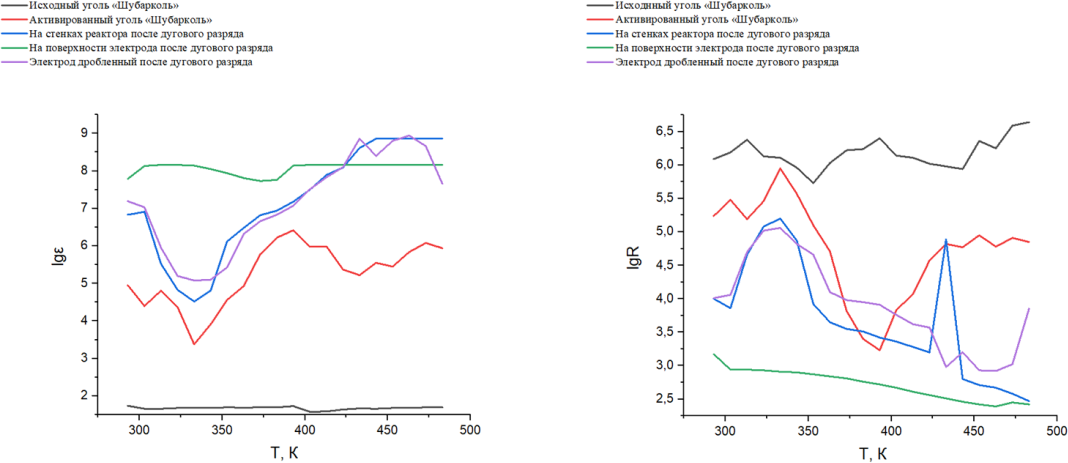
\includegraphics[width=\textwidth]{assets/65}
	\caption*{А\hspace{8cm}Б}
\end{figure}

\begin{figure}[H]
	\centering
	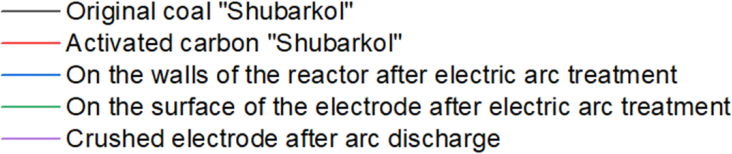
\includegraphics[width=0.5\textwidth]{assets/66}
	\caption*{Figure 13 - Dependence of dielectric constant (A) and electrical resistance (B) on temperature at a frequency of 1 kHz}
\end{figure}

\begin{multicols}{2}
Activated carbon «Shubarkol» shows that the dielectric constant of this
material has mainly average values. The maximum value of ε is achieved
at 393 K -- 2.62·10\textsuperscript{6} (1 kHz),
7.23·10\textsuperscript{5} (5 kHz) and 3.73·10\textsuperscript{5} (10
kHz). A study of the temperature dependence of electrical resistance
shows that activated carbon exhibits variable conductivity in the range
of 293-333 K, semiconductor conductivity at 333-393 K, metallic
conductivity at 393-453 K, and variable conductivity at 453-483 K.

Activated carbon "Shubarkol" after an arc discharge obtained on the
walls of the reactor at 293 K exhibits a high value of ε
(6.77·10\textsuperscript{6}) - 1 kHz, 3.72·10\textsuperscript{5} - 5 kHz
and 1.08·10\textsuperscript{5} - 10 kHz and reaches colossal values
\hspace{0pt}\hspace{0pt}at 443 - 483 K 7.20·10\textsuperscript{8} and
more (1 kHz), 2.50·10\textsuperscript{8} (5 kHz and 483 K) and
8.41·10\textsuperscript{7} (10 kHz and 483 K). A study of the
temperature dependence of the electrical resistance of material III
shows variable conductivity in the range of 293-333 K, semiconductor
conductivity at 333-423 K, and semiconductor conductivity again at
433-483 K.

Activated carbon «Shubarkol» after an arc discharge obtained on the
surface of the electrode already at lower temperatures of 293 and 343
shows gigantic values \hspace{0pt}\hspace{0pt}of dielectric constant
6.16·10\textsuperscript{7} (1 kHz), 2.90·10\textsuperscript{6} (5 kHz)
and 2.45·10\textsuperscript{6} (10 kHz) at 313 K and starting from 403 K
at 1 kHz is also ε greater than 1.44·10\textsuperscript{8} and colossal
values \hspace{0pt}\hspace{0pt}of ε are maintained (albeit with a
decrease) at frequencies of 5 and 10 kHz. Activated carbon «Shubarkol»
after an arc discharge (on the surface of the electrode) in the range of
293-463 K exhibits semiconductor conductivity, and at 463-483 K -- mixed
conductivity.

According to the temperature dependence of the dielectric constant of
Activated carbon «Shubarkol» after an arc discharge, the crushed
electrode shows that already at 293 K it shows a gigantic value at a
frequency of 1 kHz and at frequencies of 5 and 10 kHz high values
\hspace{0pt}\hspace{0pt}of dielectric constant:
1.56·10\textsuperscript{7} (1 kHz), 9.83·10\textsuperscript{5} (5 kHz)
and 2.78·10\textsuperscript{5} (10 kHz). The colossal value of ε is
achieved at 463 K and 1 kHz (8.63·10\textsuperscript{8}). The
temperature dependence of electrical resistance in the range of 293-333
K exhibits metallic conductivity, at 333-433 K - semiconductor
conductivity, and at 433-483 K - variable conductivity.
\end{multicols}

\begin{table}[H]
\caption*{Table 3 - Dependence of dielectric constant (ε) on temperature at different frequencies}
\centering
\begin{tabular}{|p{0.15\textwidth}|llllll|}
\hline
\multirow{3}{=}{Name of material} & \multicolumn{6}{l|}{The 			dielectric constant (ε)} \\ \cline{2-7} 
 & \multicolumn{2}{l|}{at 			1 kHz} & \multicolumn{2}{l|}{at 			5 kHz} & \multicolumn{2}{l|}{at 			10 kHz} \\ \cline{2-7} 
 & \multicolumn{1}{l|}{293} & \multicolumn{1}{l|}{483} & \multicolumn{1}{l|}{293} & \multicolumn{1}{l|}{483} & \multicolumn{1}{l|}{293} & 483 \\ \hline
BaTiO3 & \multicolumn{1}{l|}{1296} & \multicolumn{1}{l|}{2159} & \multicolumn{1}{l|}{1220} & \multicolumn{1}{l|}{2102} & \multicolumn{1}{l|}{561} & 2100 \\ \hline
Graphite & \multicolumn{1}{l|}{6,07*} & \multicolumn{1}{l|}{7,19*\textless{}} & \multicolumn{1}{l|}{4,04*} & \multicolumn{1}{l|}{2,56*} & \multicolumn{1}{l|}{1,15*} & 8,70* \\ \hline
On 			the walls of the reactor & \multicolumn{1}{l|}{6770953} & \multicolumn{1}{l|}{719702040˂} & \multicolumn{1}{l|}{371895} & \multicolumn{1}{l|}{249796682} & \multicolumn{1}{l|}{107561} & 84141207 \\ \hline
On 			the surface of the electrode & \multicolumn{1}{l|}{61630141} & \multicolumn{1}{l|}{143940408˂} & \multicolumn{1}{l|}{2898125} & \multicolumn{1}{l|}{69699521} & \multicolumn{1}{l|}{2453921} & 22287956 \\ \hline
Crushed 			electrode & \multicolumn{1}{l|}{15614812} & \multicolumn{1}{l|}{45948829} & \multicolumn{1}{l|}{982576} & \multicolumn{1}{l|}{2055749} & \multicolumn{1}{l|}{277845} & 601308 \\ \hline
\end{tabular}
\end{table}

\begin{multicols}{2}
As shown in Table 3, dielectric constant is inversely proportional to
frequency. Materials after an arc discharge increased their dielectric
constant. The most optimal indicator for activated carbon after an arc
discharge is obtained on the walls of the reactor. For comparison, we
gave the example of graphite and the resulting materials have a similar
dielectric constant. The band gap of the resulting materials can be
classified as narrow-gap semiconductors. Activated carbons after arc
processing are of interest for semiconductor and microcapacitor
technology.

Since the nanomaterial obtained on the walls of the reactor showed the
best results in terms of physicochemical and electrophysical properties,
the material was tested for hydrogen storage. The specific surface area
according to Langmuir theory is 112.27 m\textsuperscript{2}/g, and
according to BET - 104,08 m\textsuperscript{2}/g. For the case of 77 K,
it is also possible to determine the specific surface area and pore
distribution using DFT methods for carbon materials: total area in pores
(\textgreater= 2,91 Å) - 1 099,971 m²/g (H\textsubscript{2}). Based on
these data, the percentage of absorbed hydrogen on the adsorbent was
calculated. Nonmaterial on the walls of the reactor absorbed 0.314\%
(35.1516 cm\textsuperscript{3}/g) of the total mass.

{\bfseries Conclusions.} When conducting an experiment using an electric
arc discharge at a high current of 100 amperes, graphene and materials
containing graphene are formed both on the walls of the reactor and in
the electrode itself. The optimal degree of graphitization of 80.7\% is
achieved when graphene-containing material is formed on the walls of the
reactor after an arc discharge. The method of producing graphene through
electric arc discharge is promising and provides high purity and a
minimum number of defects in the product. It has many advantages such as
low cost, high efficiency and catalyst-free synthesis. This method is
easily scalable from laboratory conditions to industrial processes.

The use of graphene in various industries such as batteries, capacitors
and composite materials will help solve environmental problems. Graphene
has unique physical properties that make it attractive to researchers
and engineers. Some experts believe that graphene could replace silicon
transistors in the future due to its cost-effectiveness and speed.

The environmental aspect of the method lies in the ability to use coal
and carbon products to produce graphene, which will avoid the use of
chemical compounds and reagents. Thanks to this, environmentally
friendly technology with high added value of products is created.

Thus, the study made it possible to obtain important data on the
dynamics of the process of hydrogen adsorption on a porous carbon
material, its speed and efficiency. These results can be useful in the
development and optimization of hydrogen adsorption processes for
various industrial and scientific applications.

\emph{{\bfseries Financing:} The research was carried out with the
financial support of the Science Committee of the Ministry of Science
and Higher Education of the Republic of Kazakhstan (Grant No.
AR19577512. Development of scientific and technical foundations for the
production of microporous carbon nanomaterials for the separation and
storage of hydrogen).}
\end{multicols}

\begin{center}
{\bfseries References}
\end{center}

\begin{noparindent}
1.Jia X., Wei F. Advances in production and applications of carbon
nanotubes //Single-Walled Carbon Nanotubes: Preparation, Properties and
Applications.- 2019.- P. 299-333.

DOI10.1007/s41061-017-0102-2

2.Shmalko V.M.. Keush L. G. Zelenskiy O.I. Nanomaterialy iz uglya i
produktov ego piroliza // Dnepr. Lira. - 2018. -142 s. ISBN
978-966-981-030-4 (In Russian)

3.Janas D., ``Perfectly imperfect: a review of chemical tools for
exciton engineering in single-walled carbon nanotubes,'' Materials
Horizons. - 2020. - V.7. - No.11. - P. 2860 - 2881.

DOI 10.1039/D0MH00845A

4.Kukovecz Á., Kozma G., and Kónya Z. ``Multi-Walled Carbon Nanotubes,''
in Springer handbook of nanomaterials, Springer, Berlin, Heidelberg. -
2013.- P. 147-188.

DOI 10.1007/978-3-642-20595-8\_5

5.Mubarak N., Abdullah E., Jayakumar N., Sahu J. An overview on methods
for the production of carbon nanotubes// Journal of Industrial and
Engineering Chemistry. -2014. - V. 20(4).- P. 1186- 1197. DOI 1197.DOI
10.1016/j.jiec.2013.09.001

6.Osmani R.M, Kulkarni A.S, Aloorkar N.H, Bhosale R.R, Ghodake P.P,
Harkare B.R Carbon nanotubes: an impending carter in therapeutics // Int
J Pharmaceut Clin Res. - 2014.- V. 6(1) - P.84-96.

7.Hong, S., Myung, S. A flexible approach to mobility // Nature
Nanotech~2. - 2007. - P. 207-208. DOI 10.1038/nnano.2007.89

8.Diachkov P.N. Elektronnyye svoystva i primeneniye nanotrubok. --
Izd-vo: Binom. Laboratoriya znaniy. - 2014. -- 488 s. ISBN:
978-5-9963-0154-6 (In Russian)

9.Cotul U., Parmak E.D., Kaykilarli C., Saray O., Uzunsoy D., Colak O.
Development of High Purity // Few-Layer Graphene Synthesis by Electric
Arc Discharge Technique. - 2018. - V. 134. --P. 289-291. DOI
10.12693/aphyspola.134.289

10.Nan Li, Zhiyong Wang, Zujin Shi. Synthesis of Graphenes with
Arc-Discharge Method // Physics and Applications of Graphene --
Experiments.- 2011.-P.23-35.DOI 10.5772/14961

11.Yu X., Tang Z., Sun D. et al. Recent advances and remaining
challenges of nanostructured materials for hydrogen storage
applications// Prog. Mater. Sci. - 2017. - V. 88. - P. 1- 48.

DOI 10.1016/j.pmatsci.2017.03.001

12.Stoller M.D., Park S., Zhu Y. et al. // Graphene-Based
Ultracapacitors //Nano Lett. - 2008. - Vol. 8(10) - P. 3498-3502. DOI
10.1021/nl802558y.

13.Khan, U., O\textquotesingle Neill, A., Lotya, M., De, S. and Coleman,
J.N. High-Concentration Solvent Exfoliation of Graphene //Small. -2010.-
V.6. - P.864-871. DOI10.1002/smll.200902066

14. Gao W.. The Chemistry of Graphene Oxide, Eds. W. Gao, Springer,
Switzerland. -2015.-P. 61-95. DOI 10.1007/978-3-319-15500-5\_3~

15.Li N. et al. Large scale synthesis of N-doped multi-layered graphene
sheets by simple arc-discharge method // Carbon.- 2010.- Vol. 48 (1)-
P.255-259. DOI 10.1016/j.carbon.2009.09.013.

16.Çotul U. et al. Development of high purity, few-layer graphene
synthesis by electric arc discharge technique // Acta Physica Polonica
A.- 2018.-Vol.134 (1)- P.289-291.

DOI 10.12693/APhysPolA.134.289.
\end{noparindent}

\emph{{\bfseries Information about the authors}}

\begin{noparindent}
Kazankapova M.K. -PhD in Philosophy, assoc. professor, member
correspondent of the KazNANS, Leading Researcher, Head of Laboratory of
LLP "Institute of Coal Chemistry and Technology", Astana, Kazakhstan,
e-mail: maira\_1986@mail.ru;

Yermagambet B.T.{\bfseries -}Doctor of Chemical Science, Professor,
Academician of the KazNANS, Project Manager, Chief Researcher, Director
of LLP "Institute of Coal Chemistry and Technology", Astana, Kazakhstan,
e-mail: bake.yer@mail.ru;

Mendaliyev G.K.{\bfseries -}master student Eurasian National University of
L.N. Gumilyov{\bfseries ,} Astana, Kazakhstan, e-mail: ganimen@mail.ru;

Samatkyzy A.- laboratory assistant "Institute of Coal Chemistry and
Technology" LLP, Astana, Kazakhstan, e-mail: akshekina11@mail.ru;

Malgazhdarova A.B.-master student Eurasian National University of L.N.
Gumilyov{\bfseries ,} Astana, Kazakhstan, e-mail: malgazhdarova.ab@mail.ru
\end{noparindent}

\emph{{\bfseries Сведения об авторах}}

\begin{noparindent}
Казанкапова М.К. -PhD философских наук, асс. профессор, чл.-корр.
КазНАЕН, ведущий научный сотрудник, заведующий лабораторией ТОО
«Институт химии и технологии угля», Астана, Казахстан, e-mail:
maira\_1986@mail.ru;

Ермагамбет Б.Т.-доктор химических наук, профессор, академик КазНАЕН,
руководитель проекта, главный научный сотрудник, директор ТОО «Институт
химии и технологии угля», Астана, Казахстан, e-mail: bake.yer@mail.ru;

Мендалиев Г.К.- магистрант Евразийского национального университета им.
Л.Н. Гумилева, Астана, Казахстан, e-mail: ganimen@mail.ru;

Саматкызы А.{\bfseries -}лаборант ТОО «Институт химии угля и технологии»,
Астана, Казахстан, e-mail: akshekina11@mail.ru;

Малгаждарова А.Б.- магистрант Евразийского национального университета
им. Л.Н. Гумилева, Астана, Казахстан, e-mail: malgazhdarova.ab@mail.ru
\end{noparindent}
